\textbf{(3)} Considere o sistema representado abaixo, onde um compartimento de
volume V, dividido em dois volumes de \num{0,25} V e um de \num{0,50} V. Um dos volumes
menores foi preenchido com \num{0,75} mols de \ce{N2} e o outro dos volumes menores com
\num{0,25} mols de \ce{O2}, ambos a 300 K, como ilustrado abaixo. Em um certo momento, a
barreira que divide o volume é removida.  Considere ainda que os gases são
ideais.\\

\begin{figure}[H]
    \centering
    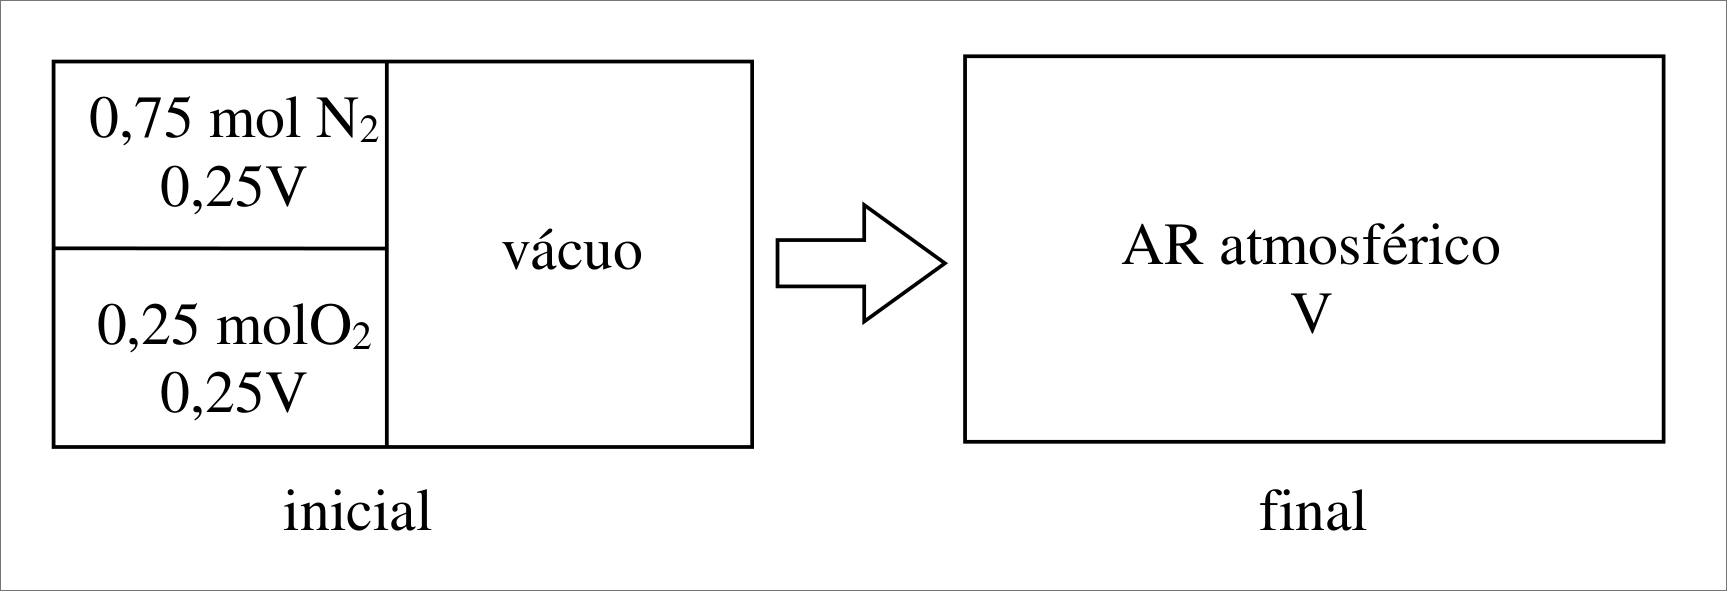
\includegraphics[width=.8\linewidth]{Q3.png}
\end{figure}

(a) Calcule a variação de entropia do \ce{N2} e do \ce{O2} entre os estados
final e inicial sabendo que a temperatura permanece constante. Indique os
cálculos a partir da derivada total apropriada.\\

(b) Calcule a variação de entropia total do sistema entre o estado inicial e
final (após a remoção das divisórias).\\

(c) Explique porque a mistura de \ce{O2} e \ce{N2}, nas condições descritas,
pode ser considerada como um processo adiabático (\(dq= 0\)).\\

    \textbf{Resposta:} A mistura de \ce{O2} e \ce{N2} nas condições descritas pode 
    ser considerada um processo adiabático (\(dq = 0\)) porque não há transferência 
    de calor entre o sistema e a vizinhança. Isso ocorre porque a temperatura 
    permanece constante (processo isotérmico) e a expansão dos gases é irreversível, 
    sem realização de trabalho útil. Como os gases são ideais e a energia interna 
    depende apenas da temperatura, a variação de energia interna (\(\Delta U\)) é zero. 
    Pela Primeira Lei da Termodinâmica,

    \[
    \Delta U = q + w,
    \]

    como \(\Delta U = 0\) e \(w = 0\) (não há trabalho contra uma pressão externa, 
    pois a expansão é livre no vácuo), conclui-se que \(q = 0\). Portanto, o processo 
    é adiabático. 

(d) Algumas vezes os alunos respondem o item a dizendo que a variação de
entropia é zero pois a entropia é definida como \(dS= dq_{\text{rev}}/T\) e,
sendo o processo adiabático (item c), \(dS\) também deveria ser zero. Explique
qual é o problema com esse raciocínio.\\

    \textbf{Resposta:} O raciocínio de que a variação de entropia é zero porque 
    \(dS = \frac{dq_{\text{rev}}}{T}\) e o processo é adiabático (\(dq = 0\)) é 
    incorreto porque ignora a natureza irreversível do processo. A definição 
    \(dS = \frac{dq_{\text{rev}}}{T}\) só se aplica a processos reversíveis. 
    Neste caso, a mistura dos gases é um processo irreversível, e a entropia deve 
    ser calculada considerando a expansão isotérmica irreversível de cada gás no 
    volume final. A entropia do sistema aumenta devido ao aumento da desordem 
    molecular, mesmo sem transferência de calor. Portanto, a variação de entropia 
    não é zero, e o erro está em aplicar uma fórmula válida apenas para processos 
    reversíveis a um processo irreversível.
